% Apresentação derivada de compressores.tex — compilar com pdflatex (2x)
\documentclass[aspectratio=169,12pt]{beamer}
\usetheme{metropolis}
\usepackage[utf8]{inputenc}
\usepackage[T1]{fontenc}
\usepackage[brazil]{babel}
\usepackage{amsmath,amssymb}
\usepackage{graphicx}
\usepackage{booktabs}

\setbeamerfont{footnote}{size=\tiny}
\newcommand{\credito}[1]{{\vspace{-0.5em}\par\tiny\textcolor{gray}{#1}\par}}

\title{Gêmeo Digital de Sistemas de Compressão Offshore}
\subtitle{Diretrizes Técnicas, Modelagem e Implementação}
\author{Engenheiro Marcelo Moreira Mejias, M.Sc.}
\date{\today}

\begin{document}

\maketitle

\begin{frame}{Agenda}
	\begin{columns}[T]
		\column{0.5\textwidth}
		\textbf{Parte I — Física e Falhas}
		\begin{itemize}
			\item O sistema de ar comprimido offshore
			\item Princípio do compressor de parafuso oil-free
			\item Componentes: transmissão, lubrificação, estágios LP/HP, intercooler, PSA
			\item Mecanismos de falha e indicadores digitais
		\end{itemize}
		\column{0.5\textwidth}
		\textbf{Parte II — O Gêmeo Digital}
		\begin{itemize}
			\item Exergia e sustentabilidade
			\item Modelagem híbrida (gray-box)
			\item EKF, VAE, PIML
			\item Otimização: MPC e PSO
			\item Diretrizes de implementação e evolução
		\end{itemize}
	\end{columns}
	\vspace{0.5em}
	\textbf{Parte III — Estudo de Caso Integrado (Cap.\ 28--29):} metodologia de calibração de parâmetros + demonstração numérica ponta a ponta.
\end{frame}

\begin{frame}{O que é um Gêmeo Digital?}
	\begin{itemize}
		\item Representação virtual \textbf{dinâmica} de um ativo físico: modelos de primeiros princípios acoplados a dados de sensores em tempo real.
		\item Diferente de uma simulação estática, \textbf{evolui com o ativo}: incorpora histórico de degradação, variações ambientais e eventos operacionais.
		\item Termo cunhado por Michael Grieves (2002); formalizado pela NASA/USAF (2012) para prognóstico de veículos aeroespaciais de alta criticidade.
	\end{itemize}
	\vfill
	\begin{alertblock}{Objetivos declarados}
		Menor consumo específico (kWh$\cdot$m$^{-3}$) $\;\bullet\;$ menor CO$_2$eq $\;\bullet\;$ manutenção preditiva baseada em condição real
	\end{alertblock}
\end{frame}

\begin{frame}{O sistema em escopo: quatro pilares}
	\centering
	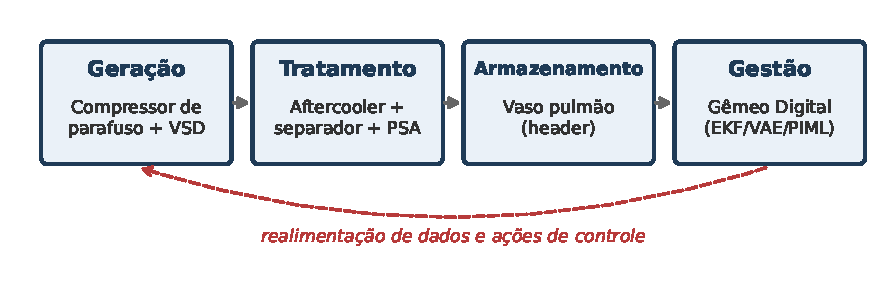
\includegraphics[width=0.5\textwidth]{figuras/fig_2_2_arquitetura.pdf}
	\begin{itemize}
		\item \textbf{Geração}: parafuso rotativo oil-free, timing gears, VSD (7--10 bar)
		\item \textbf{Tratamento}: aftercooler, separadores, PSA \quad \textbf{Armazenamento}: vasos pulmão
		\item \textbf{Gestão}: camada de dados — performance, diagnóstico, RUL — em malha fechada
	\end{itemize}
\end{frame}

\begin{frame}{Princípio do compressor de parafuso}
	\begin{columns}[T]
		\column{0.42\textwidth}
		\centering
		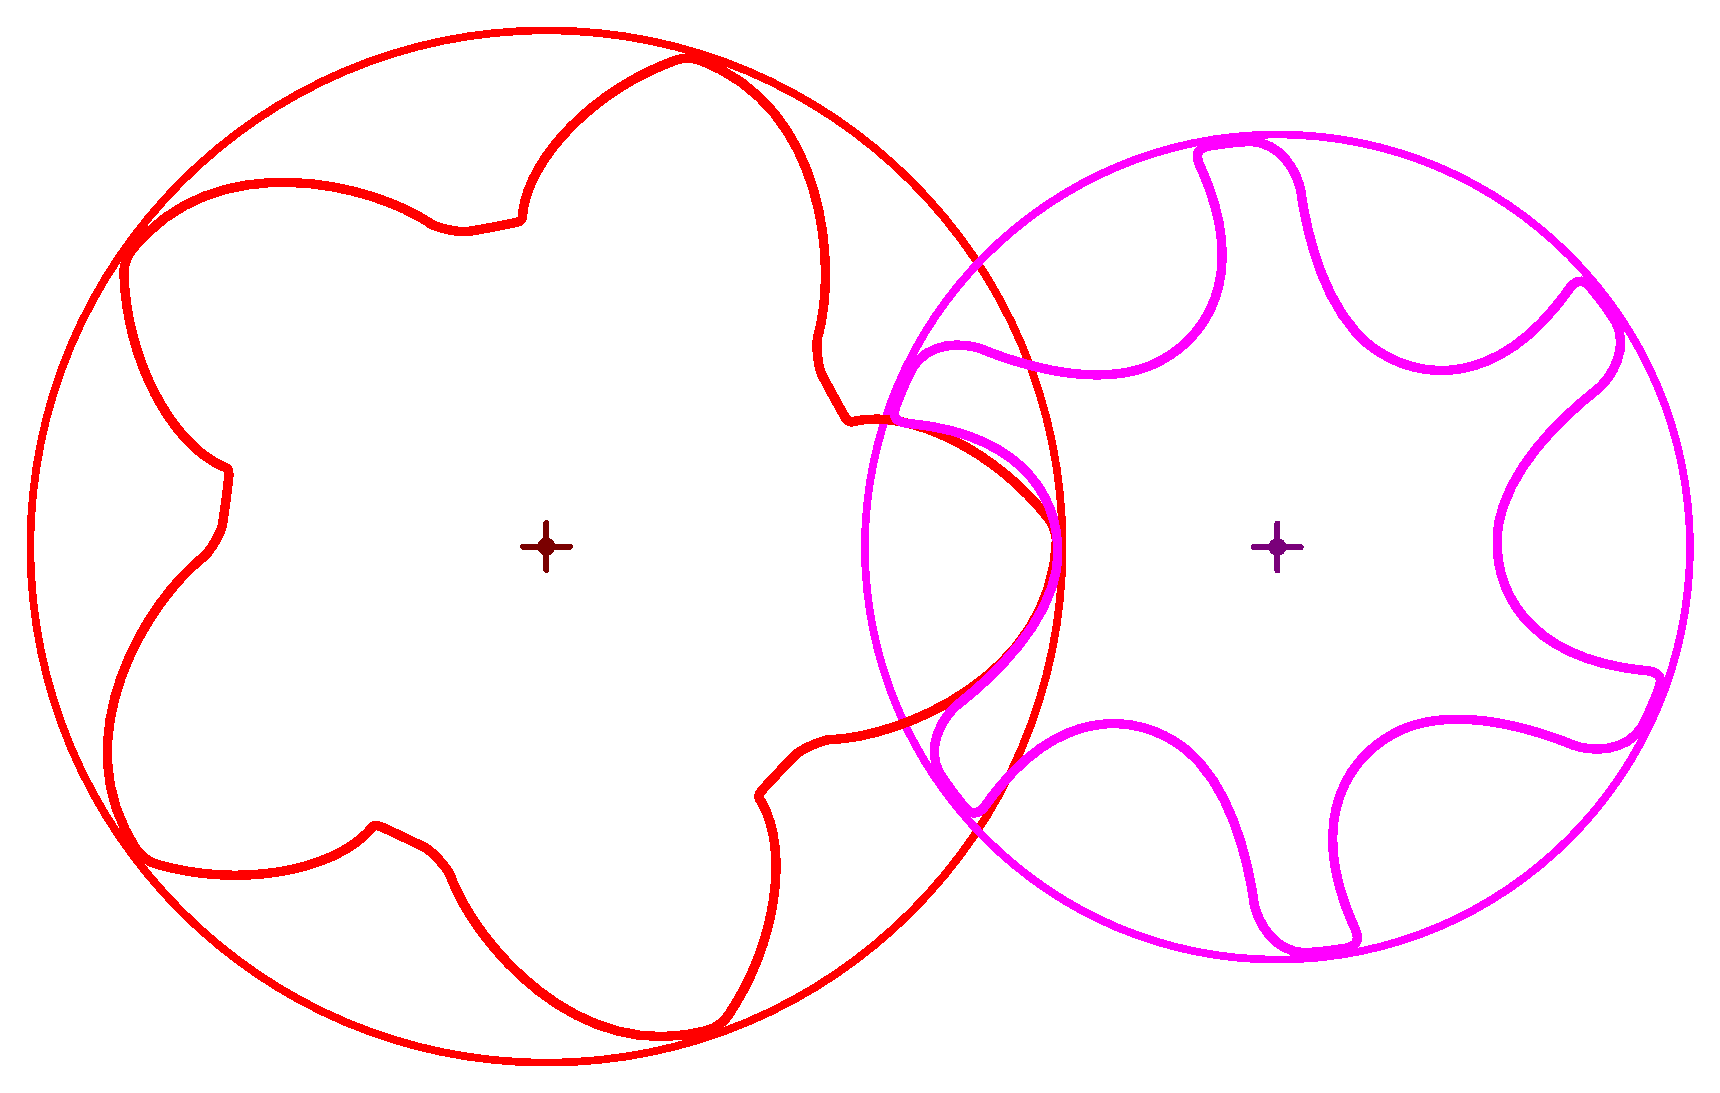
\includegraphics[width=0.85\textwidth]{figuras/fig_2_1_rotores.pdf}
		\credito{Adaptado de \textit{Asymmetric Screw Compressor Rotor Mesh}, Slashme, Wikimedia Commons, CC BY-SA 4.0.}
		\column{0.58\textwidth}
		\begin{enumerate}
			\item \textbf{Admissão}: câmara em ``V'' se abre na sucção e admite o ar.
			\item \textbf{Compressão}: o engrenamento avança pela hélice, reduzindo o volume — deslocamento positivo contínuo, sem válvulas.
			\item \textbf{Descarga}: a aresta fixa da porta define a razão volumétrica interna $V_i$.
		\end{enumerate}
		\vspace{0.3em}
		Um rotor é o \textbf{negativo} do outro: vedação contínua em toda a rotação.
	\end{columns}
\end{frame}

\begin{frame}{Oil-free: sincronismo externo obrigatório}
	\begin{columns}[T]
		\column{0.5\textwidth}
		\centering
		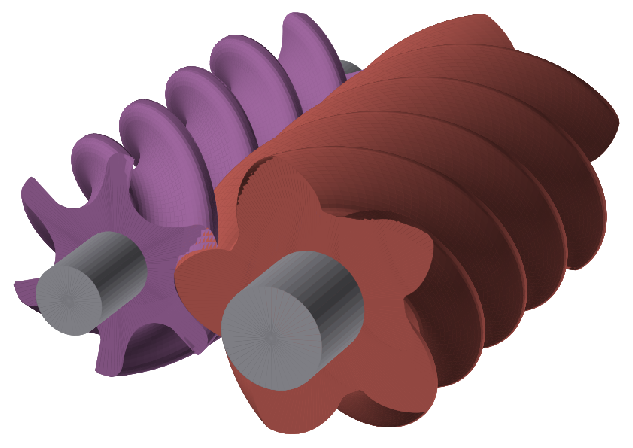
\includegraphics[width=\textwidth]{figuras/fig_3_1_parafuso3d.pdf}
		\credito{Render 3D derivado do perfil de Slashme (Wikimedia Commons, CC BY-SA 4.0), elaborado pelo autor.}
		\column{0.5\textwidth}
		\begin{itemize}
			\item Sem óleo na câmara de compressão $\Rightarrow$ sem filme para transmitir torque entre rotores.
			\item Eixos sincronizados por \textbf{engrenagens de timing}: folga constante, sem contato metal--metal.
			\item Lubrificação restrita à gearbox e aos mancais dos estágios.
			\item Dois estágios (LP e HP) com intercooler entre eles.
		\end{itemize}
	\end{columns}
\end{frame}

\begin{frame}{Ambiente offshore: desafios e normas}
	\begin{columns}[T]
		\column{0.5\textwidth}
		\textbf{Desafios (FPSOs e plataformas)}
		\begin{itemize}
			\item Salinidade: colmatagem de filtros, corrosão em trocadores
			\item Umidade elevada: mais condensado
			\item Atmosferas explosivas (IEC 60079)
			\item Rede elétrica isolada: harmônicas de VSD, flutuações de carga
		\end{itemize}
		\column{0.5\textwidth}
		\textbf{Referências normativas}
		\begin{itemize}
			\item API 619 — compressores de deslocamento positivo (O\&G)
			\item ISO 10440-1 / ISO 1217
			\item NORSOK M-501 — revestimentos
			\item ASME VIII Div.\ 1 — vasos de pressão
			\item ISO 8573-1 — qualidade do ar
		\end{itemize}
	\end{columns}
	\vfill
	\begin{alertblock}{Diretriz}
		Cada equação do modelo é rastreável a um limite normativo: o DT nunca recomenda ação fora da fronteira certificada de projeto.
	\end{alertblock}
\end{frame}

\begin{frame}{Decisão metodológica: física primeiro, IA depois}
	\begin{columns}[T]
		\column{0.5\textwidth}
		\textbf{Parte I (Cap.\ 2--14)}\\
		Cada subsistema sob três lentes:
		\begin{enumerate}
			\item O elemento de máquina
			\item Modelagem termodinâmica/mecânica (primeiros princípios)
			\item Mecanismos de falha + indicador digital
		\end{enumerate}
		\column{0.5\textwidth}
		\textbf{Parte II (Cap.\ 15--24)}\\
		Integração: EKF, VAE, PIML, MPC/PSO.
		\vspace{0.5em}
		\begin{block}{Por quê nessa ordem?}
			IA sem física explícita é um interpolador estatístico sem garantias. O PIML só penaliza violações de conservação de massa ou da 2ª Lei porque essas leis foram equacionadas antes, componente a componente.
		\end{block}
	\end{columns}
\end{frame}

\begin{frame}{Parte I em destaque: razão volumétrica interna $V_i$}
	\centering
	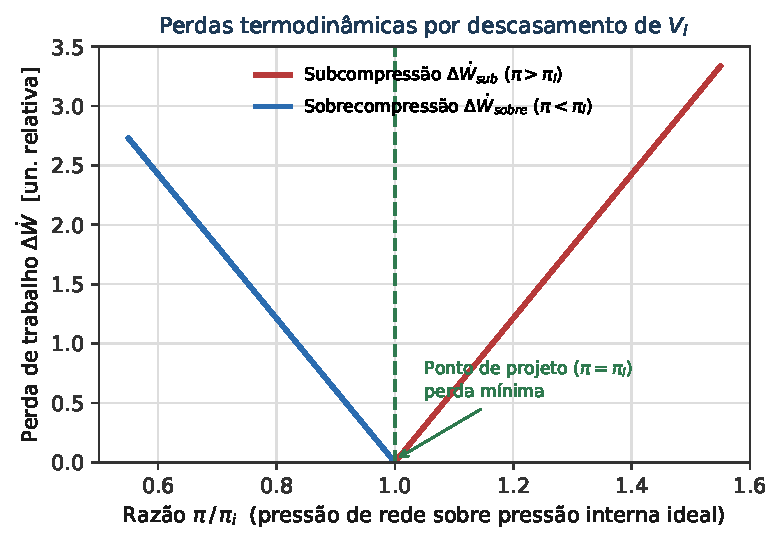
\includegraphics[width=0.42\textwidth]{figuras/fig_5_1_vi_perdas.pdf}
	\begin{itemize}
		\item Razão de pressão da rede $\neq$ projeto $\Rightarrow$ perdas por \textbf{subcompressão} ou \textbf{sobrecompressão}.
		\item O VSD desloca o ponto de operação — o DT quantifica essa perda em tempo real.
	\end{itemize}
\end{frame}

\begin{frame}{Trem de transmissão e confiabilidade}
	\begin{columns}[T]
		\column{0.5\textwidth}
		\centering
		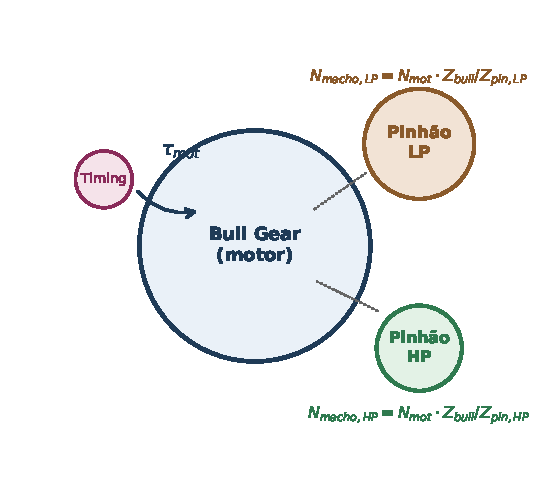
\includegraphics[width=0.68\textwidth]{figuras/fig_8_1_gearbox.pdf}
		\column{0.5\textwidth}
		\centering
		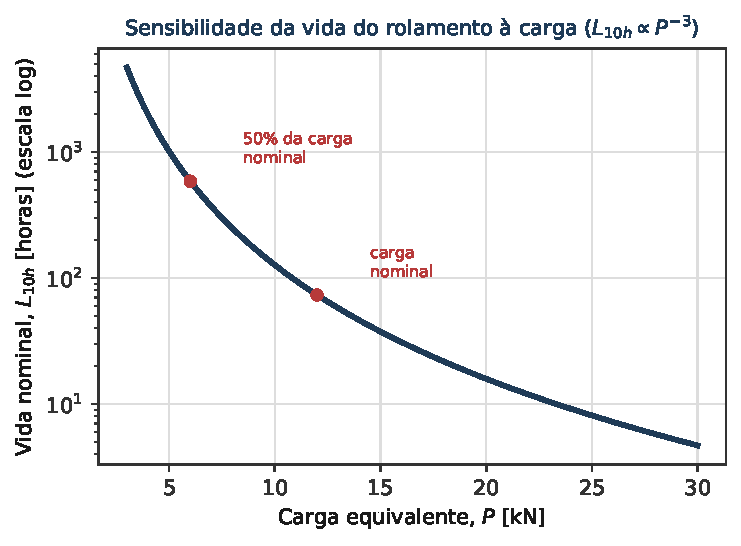
\includegraphics[width=0.68\textwidth]{figuras/fig_8_3_l10h.pdf}
	\end{columns}
	\begin{itemize}
		\item Cinemática motor $\to$ gearbox $\to$ timing gears; perdas parasitas modeladas termo a termo.
		\item Vida de rolamentos ($L_{10h}$), rotordinâmica (Campbell) e integridade de dentes formam a \textbf{matriz de falhas} com indicadores digitais.
	\end{itemize}
\end{frame}

\begin{frame}{Lubrificação e térmica dos subsistemas}
	\begin{columns}[T]
		\column{0.5\textwidth}
		\centering
		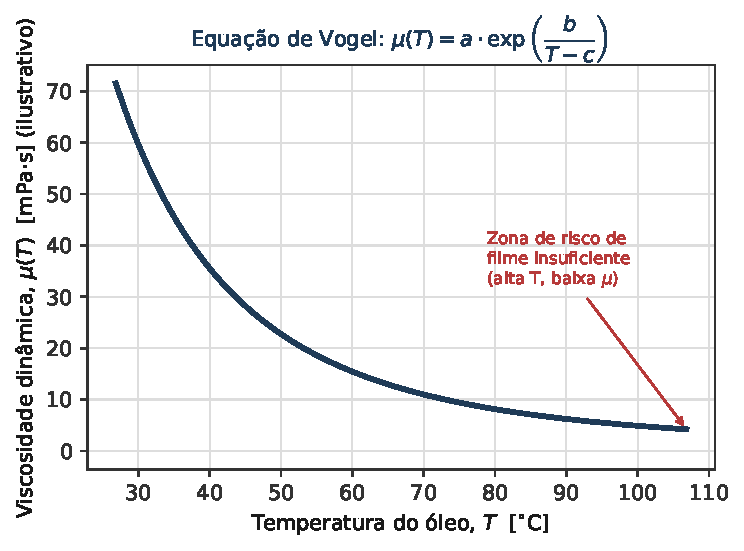
\includegraphics[width=0.78\textwidth]{figuras/fig_7_1_vogel.pdf}
		\begin{itemize}
			\item Óleo (Vogel): viscosidade cai exponencialmente com $T$ — janela estreita entre desgaste e perda de carga.
		\end{itemize}
		\column{0.5\textwidth}
		\centering
		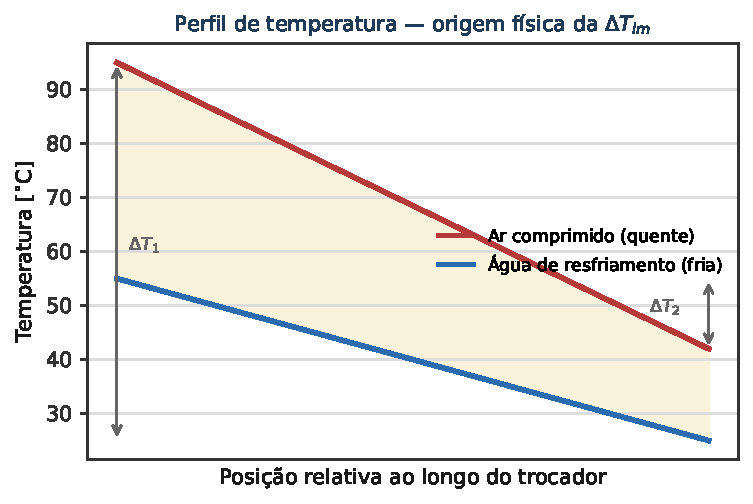
\includegraphics[width=0.78\textwidth]{figuras/fig_10_1_lmtd.pdf}
		\begin{itemize}
			\item Intercooler: efetividade e LMTD; \textit{fouling} e \textit{offloading} como falhas interna e externa.
		\end{itemize}
	\end{columns}
\end{frame}

\begin{frame}{Tratamento de ar: secagem por adsorção (PSA)}
	\begin{columns}[T]
		\column{0.45\textwidth}
		\centering
		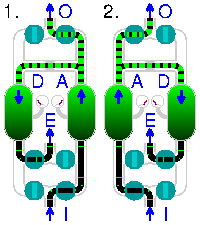
\includegraphics[width=0.85\textwidth]{figuras/fig_15_1_psa.pdf}
		\credito{Adaptado de \textit{Pressure swing adsorption principle}, Cmglee, Wikimedia Commons, CC BY-SA 4.0.}
		\column{0.55\textwidth}
		\begin{itemize}
			\item Duas torres: uma adsorve sob pressão, a outra regenera por purga de ar seco.
			\item Variável crítica: ponto de orvalho $T_{dp} \le -40\,^{\circ}$C (ISO 8573-1).
			\item O DT antecipa o \textbf{breakthrough} do leito dessecante pela taxa $dT_{dp}/dt$ — antes do limite normativo.
			\item Material selecionável (alumina, sílica, peneira molecular); regeneração como recuperação exponencial de 1ª ordem, não uma reta.
		\end{itemize}
	\end{columns}
\end{frame}

\begin{frame}{Exergia: a régua única de perdas}
	A energia se conserva (1ª Lei); a \textbf{exergia} — capacidade de realizar trabalho útil — é destruída em todo processo real (2ª Lei):
	\begin{equation*}
		\dot{I} = T_0 \cdot \dot{S}_{gen} = \sum \dot{m}_{in}\,\psi_{in} - \sum \dot{m}_{out}\,\psi_{out} - \dot{W}_{shaft}
	\end{equation*}
	\begin{itemize}
		\item Converte vazamento interno, incrustação e atrito em \textbf{Watts comparáveis} — prioriza a intervenção que mais devolve eficiência.
		\item Emissões como consequência direta: $\dot{m}_{CO_2} = \dot{W}_{total} \cdot EF_{carbon}$.
	\end{itemize}
	\begin{alertblock}{Ponto de Máxima Sustentabilidade}
		$\text{Min } \dot{S}_{gen} \implies \text{Min } \dot{m}_{CO_2}$, \quad com $T_{dp} < T_{dp,limit}$
	\end{alertblock}
\end{frame}

\begin{frame}{Modelagem híbrida (gray-box)}
	O estado real é decomposto em física explícita + resíduo aprendido:
	\begin{equation*}
		y_{\text{real}} = \underbrace{f_{\text{física}}(x, \theta)}_{\text{primeiros princípios}} + \underbrace{\epsilon_{\text{IA}}(x, \phi)}_{\text{deriva: desgaste, fouling}}
	\end{equation*}
	\begin{itemize}
		\item $f_{\text{física}}$: equações politrópicas, balanços de massa/energia/exergia (Parte I).
		\item $\epsilon_{\text{IA}}$: captura o que a física idealizada não descreve.
		\item Restrição permanente de consistência: $\dot{I} = T_0\,\dot{S}_{gen} \ge 0$.
	\end{itemize}
\end{frame}

\begin{frame}{Estimação de estados: Filtro de Kalman Estendido}
	\begin{columns}[T]
		\column{0.55\textwidth}
		\centering
		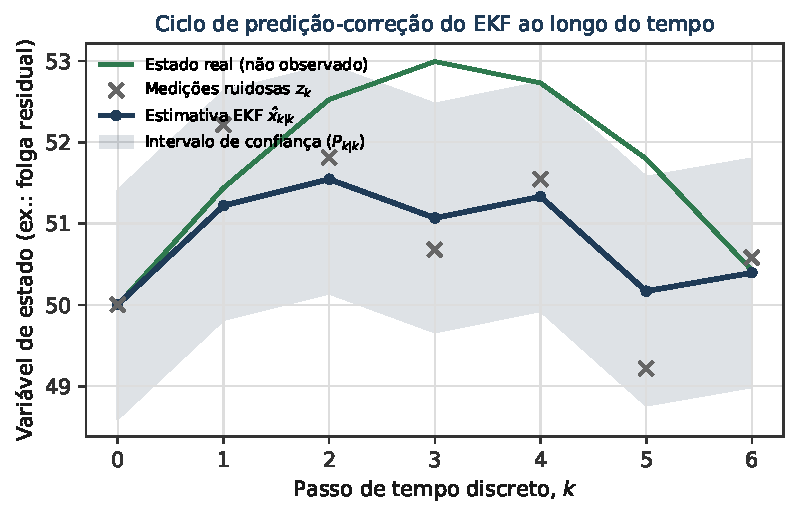
\includegraphics[width=\textwidth]{figuras/fig_21_1_ekf.pdf}
		\column{0.45\textwidth}
		\begin{itemize}
			\item Estima estados \textbf{não instrumentáveis}: folga residual $\delta$, eficiência $\eta_{is}$, incrustação $R_f$.
			\item Ciclo predição--correção: o modelo físico prevê, a medição ruidosa corrige via ganho de Kalman.
			\item A banda de incerteza $P_{k|k}$ se estreita a cada correção (leitura portátil/wireless: $\mathcal{R}$ inflada por $\kappa_{\text{port}}$).
		\end{itemize}
	\end{columns}
\end{frame}

\begin{frame}{Redução de dimensionalidade: Autoencoder Variacional}
	28 variáveis monitoradas $\to$ espaço latente $\ell \in \mathbb{R}^d$, $d \ll 28$ (Kingma \& Welling, 2013):
	\begin{equation*}
		L_{\text{VAE}} = \underbrace{\| z - \hat{z} \|^2}_{\text{erro de reconstrução}} + \beta \cdot \underbrace{D_{KL}[\mathcal{N}(\mu,\sigma) \,\|\, \mathcal{N}(0,1)]}_{\text{regularização}}
	\end{equation*}
	\begin{itemize}
		\item O erro de reconstrução $E_{\text{rec}}$ atua como \textbf{sensor virtual de saúde}: se $E_{\text{rec}} > \tau$, dispara o diagnóstico da variável causadora.
		\item $\beta$ calibrado contra falhas históricas — alto demais mascara desvios reais.
	\end{itemize}
\end{frame}

\begin{frame}{Physics-Informed Machine Learning}
	A física entra \textbf{na função de perda} da rede neural (Raissi et al., 2019):
	\begin{equation*}
		L_{\text{PIML}} = \frac{1}{N}\sum (y - \hat{y})^2 + \lambda \cdot \frac{1}{N_f}\sum \| \mathcal{F}(\hat{y}) \|^2
	\end{equation*}
	\begin{itemize}
		\item $\mathcal{F}$: resíduo das equações diferenciais — ex.\ conservação de massa no estágio HP: $\mathcal{F} = \dot{m}_{in} - \dot{m}_{out} - \frac{d}{dt}(\rho V)$.
		\item Predições termodinamicamente impossíveis são \textbf{penalizadas no treinamento}.
		\item $\lambda$ por validação cruzada: excesso ignora os dados, falta permite violações físicas.
	\end{itemize}
\end{frame}

\begin{frame}{Camada de decisão: MPC e PSO}
	\begin{columns}[T]
		\column{0.55\textwidth}
		\textbf{MPC — controle em tempo real}
		\begin{equation*}
			\text{Min } J = \sum_{k=0}^{H} \left[ \dot{W}_{\text{elec}}(k) + \beta \cdot \dot{I}(k) \right]
		\end{equation*}
		sujeito a:
		\begin{equation*}
			\begin{cases} \sigma_{b,\text{real}} < \sigma_{b,\text{adm}} & \text{(integridade)} \\ T_{dp} \le -40\,^{\circ}\text{C} & \text{(ISO 8573-1)} \end{cases}
		\end{equation*}
		\column{0.45\textwidth}
		\textbf{PSO — sintonia offline}
		\begin{itemize}
			\item Metaheurística de enxame (Kennedy \& Eberhart, 1995)
			\item Hiperparâmetros e setpoints globais em superfícies não convexas
		\end{itemize}
		\begin{alertblock}{Papéis complementares}
			PSO no laço de tempo real introduz latência incompatível com a proteção mecânica.
		\end{alertblock}
	\end{columns}
\end{frame}

\begin{frame}{Workflow de implementação}
	\begin{enumerate}
		\item \textbf{Ingestão}: limpeza, outliers (Isolation Forest), sincronização de $P, T, V, I$, vibração
		\item \textbf{Inferência}: EKF (estado de degradação) + VAE (filtragem de ruído)
		\item \textbf{Integridade e exergia}: $\sigma_b$ e $\dot{I}$ calculados simultaneamente
		\item \textbf{Prognóstico}: RUL + prescrição de ajuste de carga ou manutenção
	\end{enumerate}
	\vfill
	\begin{columns}[T]
		\column{0.5\textwidth}
		\textbf{Edge (na plataforma)}
		\begin{itemize}
			\item Alta frequência: harmônicos de vibração, EKF
		\end{itemize}
		\column{0.5\textwidth}
		\textbf{Cloud}
		\begin{itemize}
			\item Treinamento do VAE, otimização de longo prazo
		\end{itemize}
	\end{columns}
\end{frame}

\begin{frame}{Evolução do Gêmeo Digital: um organismo vivo}
	\begin{itemize}
		\item \textbf{Quantificação de incerteza}: propagação das incertezas de sensores até os KPIs ($u(\dot{I})$); camadas bayesianas no PIML.
		\item \textbf{Explicabilidade (XAI)}: valores de SHAP mostram ao operador \textit{qual sensor} pesou no diagnóstico; trajetória de degradação visualizada no espaço latente.
		\item \textbf{MLOps}: detecção de drift pelo $E_{\text{rec}}$ do VAE; retreinamento automatizado após manutenções que alterem o ativo físico.
	\end{itemize}
	\vfill
	\begin{alertblock}{Diretriz}
		Calibração contínua via EKF + consistência física via PIML = segurança estrutural e eficiência exergética em tempo real.
	\end{alertblock}
\end{frame}

\begin{frame}{Parte III: calibrar antes de detectar (Cap.\ 28)}
	Parâmetros nunca medidos nesta máquina entram no vetor de estado do EKF:
	\begin{equation*}
		x_{\text{aug}} = \begin{bmatrix} x \\ \Lambda \end{bmatrix}, \qquad \Lambda = \begin{bmatrix} K \\ \eta_{\text{mec}} \\ \zeta_{\text{ref}} \\ \zeta_{\text{valv}} \end{bmatrix}
	\end{equation*}
	\begin{itemize}
		\item Calibrados numa \textbf{janela saudável}; depois, deriva lenta rastreada com $Q_\Lambda$ pequeno.
		\item Protocolo de 4 categorias classifica todo parâmetro: medido, inferível, calibrável ou desconhecido.
		\item Catálogo: 59 mecanismos de falha $\to$ algoritmo mais indicado — sem inflar a IA onde um limiar já basta.
	\end{itemize}
\end{frame}

\begin{frame}{Parte III: o cenário integrado em ação (Cap.\ 29)}
	Desgaste gradual da folga $\delta$ do estágio LP ao longo de 6 semanas — cada sintoma isolado \textbf{abaixo} do limiar H/HH individual:
	\begin{itemize}
		\item \textbf{EKF}: $\hat\delta/L$ converge de $0{,}0020$ para $\approx 0{,}0091$.
		\item \textbf{VAE}: $E_{\text{rec}}$ cruza o limiar na 5ª semana — mesmo sem nenhuma variável isolada fora de faixa.
		\item \textbf{PIML}: testado contra hipóteses alternativas (incrustação, viés de $T_{amb}$) — isola a causa-raiz.
		\item \textbf{MPC}: decide entre antecipar manutenção ou reduzir setpoint, com os dois custos lado a lado.
	\end{itemize}
	\begin{alertblock}{Prognóstico}
		$RUL_\delta \approx 9$ semanas (IC 95\%: 6--14) — um alarme convencional, linha por linha, não veria nada.
	\end{alertblock}
\end{frame}

\begin{frame}{Não é só teoria: simulador funcional (\texttt{aplicativo/})}
	Implementação real (Python/NumPy/PyTorch/SciPy) de cada algoritmo da Parte II, não pseudocódigo — 77 testes automatizados, 6 abas interativas (Streamlit):
	\begin{itemize}
		\item \textbf{EKF, VAE, PIML, MPC, PSO}: os cinco rodam de fato, ao lado da simulação do trem.
		\item \textbf{Identificação de $K$}: EKF aumentado (online), PIML (offline) e, agora, calibração em lote via Levenberg-Marquardt — sem filtro nem rede.
		\item Toda equação no código cita o número do livro — rastreável ao texto, não uma reimplementação paralela.
	\end{itemize}
	\begin{alertblock}{Achado real do processo}
		Portar as equações para código expôs 3 erros de unidade no livro (Eqs.\ 9.8, 11.6, 15.7), corrigidos em ambos.
	\end{alertblock}
\end{frame}

\begin{frame}{Síntese}
	\begin{equation*}
		\boxed{\;y_{\text{real}} = f_{\text{física}}(x) + \epsilon_{\text{IA}}(x) \quad \text{via EKF, VAE, PIML e MPC}\;}
	\end{equation*}
	\vfill
	\begin{itemize}
		\item A física não é complemento decorativo da IA — é a \textbf{restrição que a torna confiável} para operar offshore.
		\item Otimização energética nunca compromete a integridade estrutural: restrições normativas embutidas no otimizador.
		\item Resultado: menor consumo específico, menor CO$_2$eq e manutenção baseada em condição real.
	\end{itemize}
	\vfill
	\centering
	\small Documento completo: \textit{Gêmeo Digital de Sistemas de Compressão Offshore — Diretrizes Técnicas, Modelagem e Implementação} (166 p.)
\end{frame}

\end{document}
